\documentclass{ximera}
\input{../preamble.tex}
\author{Anastasiia Holovchenko \and Anna Davis (project advisor)} \title{Central Limit Theorem} 
\begin{document}
\begin{abstract}
\end{abstract}
\maketitle

\begin{example}\label{ex:cheesecake}
A restaurant claims that their cheesecake dessert contains 400 calories with a known population standard deviation of 25 calories. After an inspection, a food critic has suspected that the desert contains more calories than the restaurant claims and decided to take a sample of 100 cheesecakes to test their claim. The critic finds out that the sample mean is 410 calories. Answer the questions below:

\begin{question} 
Please identify the following:
\begin{enumerate}
    \item $\mu$ (presumed population mean) $= \answer{400}$
    \item $\sigma$ (population standard deviation) $= \answer{25}$
    \item $\bar{x}$ (sample mean) $=\answer{410}$
    \item $n$ (sample size) $= \answer{100}$
\end{enumerate}
\end{question}

\begin{question} Select the correct formula for calculating standard deviation for a sampling distribution.

\begin{multipleChoice}  
    \choice{$\sigma_{\bar{x}} = \sigma(n+1)/\sqrt{n}$}  
    \choice[correct]{$\sigma_{\bar{x}} =\sigma/\sqrt{n}$}  
    \choice{$\sigma  = \sigma_{\bar{x}} /\sqrt{n}$}  
    \choice{$\sigma = \frac{b-a}{\sqrt{12}}$}  
\end{multipleChoice} 

\end{question}

\begin{question} Using the correct formula please determine the value of standard deviation for the sampling distribution:
$$\mbox{St. dev. for sampling distribution:}\quad\sigma_{\bar{x}}= \answer{2.5}$$
\end{question}

\begin{question} Pick the correct graph that represents the sampling distribution, assuming that the mean is 400 calories [MAYBE MAKE A VIDEO HERE ON HOW TO MAKE THE GRAPH]

\begin{multipleChoice}
\choice{
      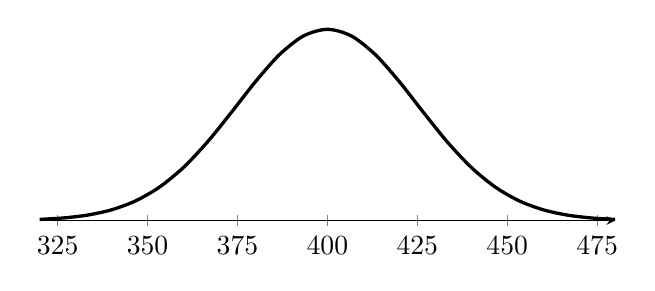
\begin{tikzpicture}
        \begin{axis}[
          domain=320:480,
          xmin=320, xmax=480,
          ymin=-0.01, ymax=0.03,
          width=3.5in,
          xtick={325,350, 375,400,425,450,475},
            xticklabels={$325$,$350$,$375$,$400$, $425$,$450$,$475$},
           % ytick style={draw=none},
            %yticklabels={},
            axis x line=center,
            axis y line=none,
          %axis lines =middle, xlabel={}, ylabel={},
          %every axis y label/.style={at=(current axis.above origin),anchor=south},
           every axis x label/.style={at=(current axis.right of origin),anchor=west},
          ]
      \addplot [very thick,  smooth] {(e^(-0.5*((x-400)/25)^2))/(((2*pi)^0.5)*25)};
      %    \node at (axis cs:320, 0.025 ) [anchor=west] {$A$};
          \end{axis}
        \end{tikzpicture}
}
\choice[correct]{
       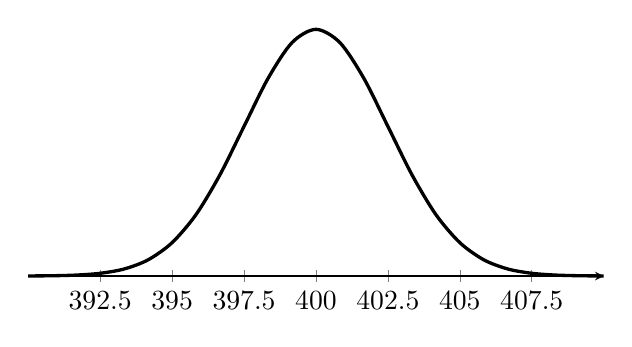
\begin{tikzpicture}
        \begin{axis}[
          domain=390:410,
          xmin=390, xmax=410,
          ymin=-0.01, ymax=0.3,
          width=3.5in,
          xtick={392.5, 395, 397.5,400,402.5,405, 407.5},
            xticklabels={$392.5$,$395$,$397.5$,$400$, $402.5$,$405$,$407.5$},
           % ytick style={draw=none},
            %yticklabels={},
            axis x line=center,
            axis y line=none,
          %axis lines =middle, xlabel={}, ylabel={},
          %every axis y label/.style={at=(current axis.above origin),anchor=south},
           every axis x label/.style={at=(current axis.right of origin),anchor=west},
          ]
      \addplot [very thick,  smooth] {(e^(-0.5*((x-400)/2.5)^2))/(((2*pi)^0.5)*2.5)};
          %\node at (axis cs:395, 0.25 ) [anchor=west] {$B$};
          \end{axis}
        \end{tikzpicture}
        }
        \choice{
        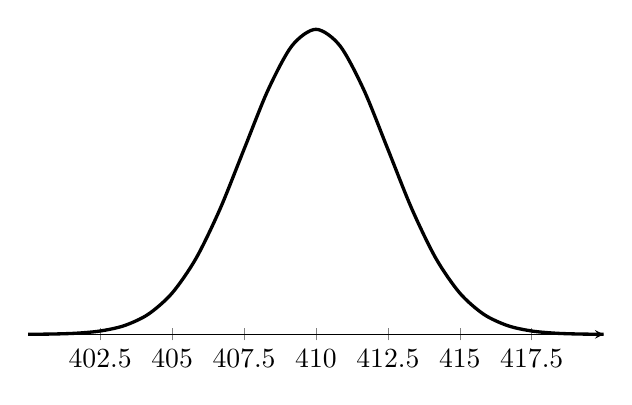
\begin{tikzpicture}
        \begin{axis}[
          domain=400:420,
          xmin=400, xmax=420,
          ymin=-0.01, ymax=0.03,
          width=3.5in,
          xtick={402.5, 405, 407.5,410,412.5,415,417.5},
            xticklabels={$402.5$,$405$,$407.5$,$410$, $412.5$,$415$,$417.5$},
           % ytick style={draw=none},
            %yticklabels={},
            axis x line=center,
            axis y line=none,
          %axis lines =middle, xlabel={}, ylabel={},
          %every axis y label/.style={at=(current axis.above origin),anchor=south},
           every axis x label/.style={at=(current axis.right of origin),anchor=west},
          ]
      \addplot [very thick,  smooth] {(e^((-(x-410)^2)/(2*2.5^2)))/(2*pi*2.5^2)};
         % \node at (axis cs:405, 0.025 ) [anchor=west] {$C$};
          \end{axis}
        \end{tikzpicture}
        }
        \choice{
        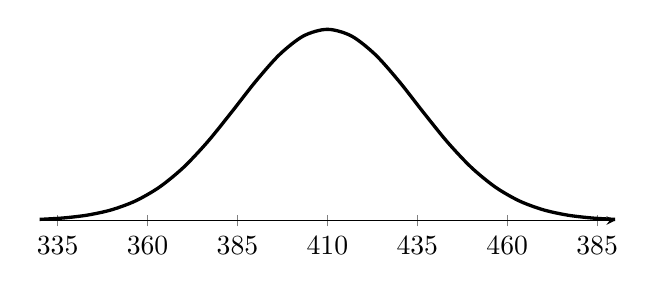
\begin{tikzpicture}
        \begin{axis}[
          domain=330:490,
          xmin=330, xmax=490,
          ymin=-0.01, ymax=0.03,
          width=3.5in,
          xtick={335,360,385,410,435,460,485},
            xticklabels={$335$,$360$,$385$,$410$, $435$,$460$,$385$},
           % ytick style={draw=none},
            %yticklabels={},
            axis x line=center,
            axis y line=none,
          %axis lines =middle, xlabel={}, ylabel={},
          %every axis y label/.style={at=(current axis.above origin),anchor=south},
           every axis x label/.style={at=(current axis.right of origin),anchor=west},
          ]
      \addplot [very thick,  smooth] {(e^(-0.5*((x-410)/25)^2))/(((2*pi)^0.5)*25)};
         % \node at (axis cs:360, 0.025 ) [anchor=west] {$D$};
          \end{axis}
        \end{tikzpicture}
 }
\end{multipleChoice}
\end{question}

\begin{question}
Assuming that the restaurant is telling the truth about having the average calorie count of 400, how likely is a sample of 100 cheesecakes to have an average calorie count of 410 or greater?
\begin{multipleChoice}
\choice{Likely}
\choice{Somewhat likely}
\choice{Unlikely}
\choice[correct]{Highly unlikely}
\end{multipleChoice}
\end{question}
\begin{question}
Do you think the restaurant is being truthful about the average calorie count in their cheesecake?
\begin{multipleChoice}
\choice{Yes}
\choice[correct]{No}
\end{multipleChoice}
\end{question}

\end{example}

\begin{example}
A potato chips company claims that on average their package contains 200 grams of potato chips. Based on the many years of testing, it is known that the population standard deviation is 10 grams and the amounts are normally distributed. Suppose that the company headquarters suspects that the manufacturer is routinely under-filling the packs of chips to cut the production cost. The company headquarters sends an inspector to the plant to find out what’s going on. The inspector picks up 25 random bags of potato chips from conveyor and finds out that the average weight of bags is 195 grams. 

\begin{question}
Please determine the value of standard deviation for the sampling distribution:
$$\mbox{St. dev. for sampling distribution:}\quad\sigma_{\bar{x}}= \answer{2}$$
\end{question}

\begin{question}
Please chose the correct graph for the sampling distribution:
\begin{image}
    \begin{tabular}{cc}
      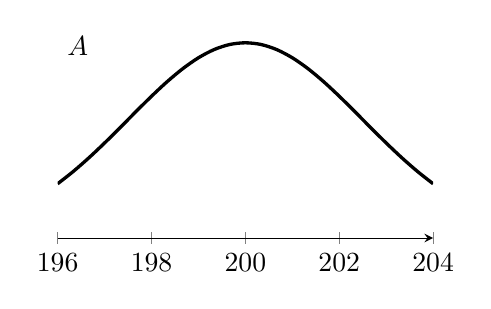
\begin{tikzpicture}
        \begin{axis}[
          domain=196:204,
          xmin=196, xmax=204,
          ymin=-0.01, ymax=0.03,
          width=2.5in,
          xtick={196, 198,200,202,204},
            xticklabels={$196$,$198$,$200$, $202$,$204$},
           % ytick style={draw=none},
            %yticklabels={},
            axis x line=center,
            axis y line=none,
          %axis lines =middle, xlabel={}, ylabel={},
          %every axis y label/.style={at=(current axis.above origin),anchor=south},
           every axis x label/.style={at=(current axis.right of origin),anchor=west},
          ]
      \addplot [very thick,  smooth] {(e^((-(x-200)^2)/(2*2.5^2)))/(2*pi*2.5^2)};
          \node at (axis cs:196, 0.025 ) [anchor=west] {$A$};
          \end{axis}
        \end{tikzpicture}
      &
      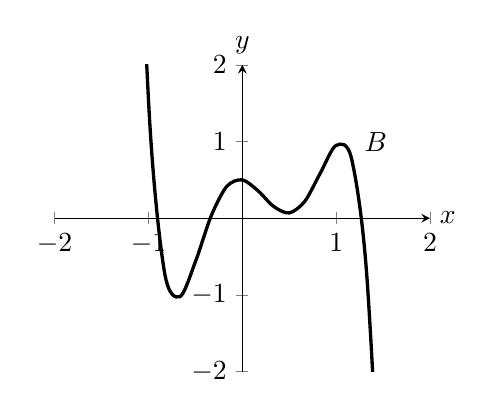
\begin{tikzpicture}
        \begin{axis}[
          domain=-2:2,
          xmin=-2, xmax=2,
          ymin=-2, ymax=2,
          width=2.5in,
          axis lines =middle, xlabel=$x$, ylabel=$y$,
          every axis y label/.style={at=(current axis.above origin),anchor=south},
          every axis x label/.style={at=(current axis.right of origin),anchor=west},
          ]
      \addplot [very thick,  smooth] {-5*x^5+5*x^4+5*x^3-4.25*x^2-.3*x +.5};
          \node at (axis cs:1.2, 1 ) [anchor=west] {$B$};
        \end{axis}
      \end{tikzpicture}\\
      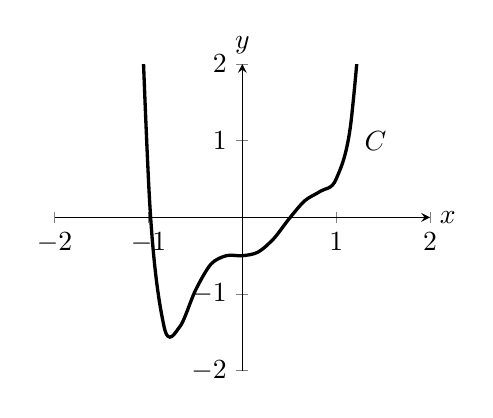
\begin{tikzpicture}
        \begin{axis}[
          domain=-2:2,
          xmin=-2, xmax=2,
          ymin=-2, ymax=2,
          width=2.5in,
          axis lines =middle, xlabel=$x$, ylabel=$y$,
          every axis y label/.style={at=(current axis.above origin),anchor=south},
          every axis x label/.style={at=(current axis.right of origin),anchor=west},
          ]
      \addplot [very thick, smooth] {5*x^6-5*x^5-5*x^4+5*x^3+x^2 -.5};
          \node at (axis cs:1.2, 1 ) [anchor=west] {$C$};
        \end{axis}
      \end{tikzpicture}
      &
      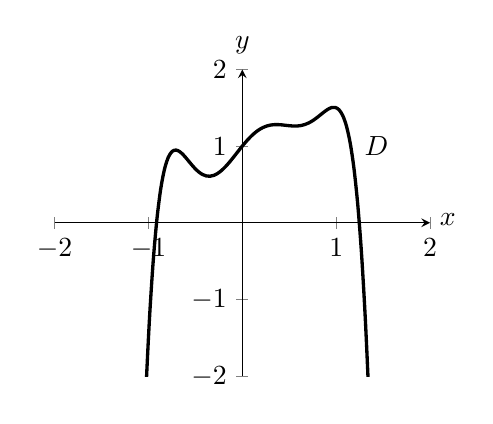
\begin{tikzpicture}
        \begin{axis}[
          domain=-2:2,
          xmin=-2, xmax=2,
          ymin=-2, ymax=2,
          width=2.5in,
          axis lines =middle, xlabel=$x$, ylabel=$y$,
          every axis y label/.style={at=(current axis.above origin),anchor=south},
          every axis x label/.style={at=(current axis.right of origin),anchor=west},
          ]
      \addplot [very thick, smooth,samples=100] {-5*x^6+5*x^5+5*x^4-5*x^3-x^2+1.5*x+1};
          \node at (axis cs:1.2, 1 ) [anchor=west] {$D$};
        \end{axis}
      \end{tikzpicture}
    \end{tabular}
  \end{image}

\end{question}
\end{example}



\begin{example}
Suppose a company manufactures snack bars. The company claims that the average wight of their granola bar is 130 grams and it's known that the population standard deviation is 6. After a routine check a mechanic stated that the machine might be broken and the weight of the granola bar is definitely not 130 grams. The company decided to test mechanics claim and took a random sample of 36 granola bars. The average weight turned out to be 133 grams.

\begin{question}
Please determine the value of standard deviation for the sampling distribution:
$$\mbox{St. dev. for sampling distribution:}\quad\sigma_{\bar{x}}= \answer{1}$$
\end{question}

\begin{question}
What is the acceptable range of the weight of the granola bar:
If we were to take thousands of samples each containing 36 bars, approximately $68\%$ of the samples would lie in what range?

\begin{hint}
Use the Empirical rule.
\end{hint}
\begin{multipleChoice}
\choice[correct]{129 - 131 grams}
\choice{124 - 136 grams}
\choice{128 - 132 grams}
\choice{127 - 133 grams}
\end{multipleChoice}
\end{question}

\begin{question}
How many standard deviations away from the mean is considered "highly unlikely"?
\begin{multipleChoice}
\choice{1 std}
\choice{2 std}
\choice[correct]{3 std}
\end{multipleChoice}
\end{question}

\begin{question}
Please specify how likely is the mean of 130 grams per bag to occur:
\begin{multipleChoice}
\choice{Likely}
\choice{Somewhat likely}
\choice[correct]{Unlikely}
\end{multipleChoice}
\end{question}

Sample question.  What is the answer?
$$\text{Solution: }\answer{4}$$

\end{example}


\begin{example}
Farmer Joe is looking to sell his farm along with animals. Emily is interested in buying the farm. To make the offer sound more appealing, Farmer Joe states that his chicken on average lay 10 eggs per week (with a std of 1), while the national average is only 6 eggs per week. Emily wants to test Joe’s claim and decides to see herself how many eggs Joe's chickens will produce in 1 week. Among 9 Joe's chickens, the average number of eggs per week turned out to be 9.5 . 

\begin{question}
Please identify the following:
[I AM CONFUSED MYSELF HERE TO BE HONEST]
\begin{enumerate}
    \item $\mu$ (presumed population mean) $= \answer{6}$
    \item $\sigma$ (population standard deviation) $= \answer{1}$
    \item $\bar{x}$ (sample mean) $=\answer{9.5}$
    \item $n$ (sample size) $= \answer{9}$
\end{enumerate}
\end{question}

\begin{question}
How likely is that the Farmer Joe tells the truth about his chickens?
\begin{multipleChoice}
\choice{Likely}
\choice[correct]{Somewhat likely}
\choice{Unlikely}
\end{multipleChoice}
\end{question}


\end{example}




\end{document} 